\section{Pointer to struct Variables}
\label{sec:structs}
\begin{frame}<beamer>
    \frametitle{Outline}
    \tableofcontents[currentsection]
\end{frame}

\begin{frame}[fragile]{Pointer to struct Type Variable (1)}
\begin{itemize}
	\item {The declaration of pointer to \textcolor{blue}{struct} type is similar as pointer to primitive type and array}
\end{itemize}
\begin{lstlisting}[basicstyle=\normalsize, xleftmargin=0.05\linewidth, linewidth=0.85\linewidth]
struct STD {
  char name[16];
  float gpa;
};
int main()
{
   struct STD std1 = {"Peter", 3.8};
   struct STD *p = &std1;
   printf("Name: %s\n", (*p).name);
   printf("GPA: %f\n", (*p).gpa);
   return 0;
}
\end{lstlisting}
\end{frame}

\begin{frame}[fragile]{Pointer to struct Type Variable (1)}
\begin{itemize}
	\item {The declaration of pointer to \textcolor{blue}{struct} type is similar as pointer to primitive type and array}
\end{itemize}
\begin{lstlisting}[basicstyle=\normalsize, xleftmargin=0.1\linewidth, linewidth=0.9\linewidth]
struct STD {
  char name[16];
  float gpa;
};
int main()
{
   struct STD std1 = {"Peter", 3.8};
   struct STD *p = &std1;
   printf("Name: %s\n", (*p).name);
   printf("GPA: %f\n", (*p).gpa);
   return 0;
}
\end{lstlisting}
\end{frame}

\begin{frame}[fragile]{Pointer to struct Type Variable (2): explained}
\vspace{0.15in}
\begin{figure}
	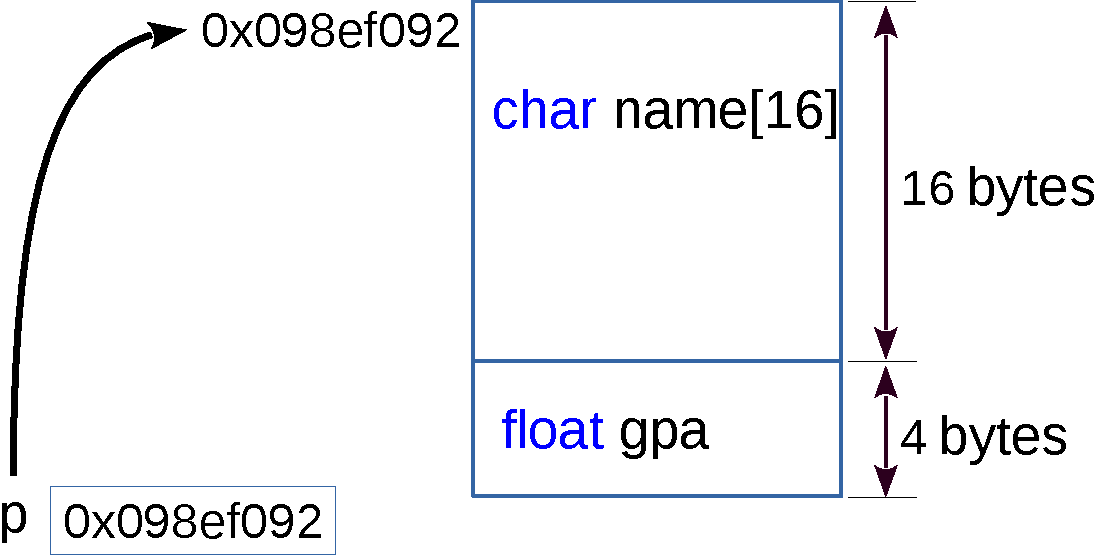
\includegraphics[width=0.55\linewidth]{figs/p2struct.pdf}
\end{figure}
\begin{itemize}
	\item {Pointer keeps the starting address of the struct type variable}
	\item {\textcolor{blue}{sizeof}(p) = ?}
\end{itemize}
\end{frame}

\begin{frame}[fragile]{Pointer to struct Type Variable (3): explained}
\vspace{0.15in}
\begin{figure}
	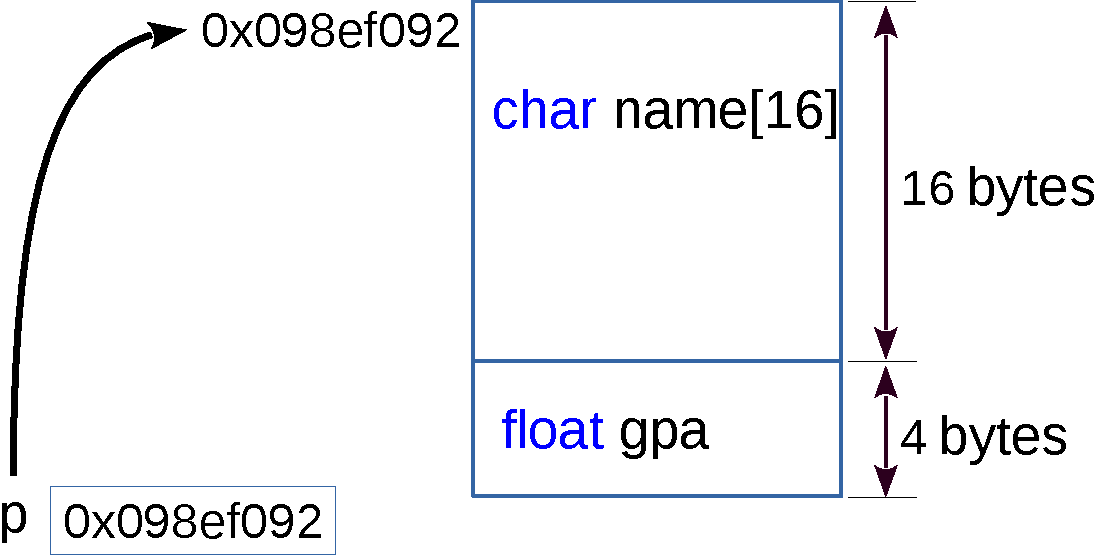
\includegraphics[width=0.55\linewidth]{figs/p2struct.pdf}
\end{figure}
\begin{itemize}
	\item {Pointer keeps the starting address of the struct type variable}
	\item {\textcolor{blue}{sizeof}(p) = ?}
	\item {Notice that the address is only 4 bytes (32 bits system)}
\end{itemize}
\end{frame}

\begin{frame}[fragile]{Pointer to struct Type Variable}
\vspace{-0.2in}
\begin{columns}
\begin{column}{0.46\linewidth}
\begin{lstlisting}
struct STD {
  char name[16];
  float gpa;
};
typedef struct STD STDT;
int main()
{
 STDT std1 = {"Peter", 3.8};
 struct STD *p = &std1;
 printf("%s\n", (*p).name);
 printf("%f\n", (*p).gpa);
 return 0;
}
\end{lstlisting}
\end{column}
\begin{column}{0.46\linewidth}
\begin{lstlisting}
struct STD {
  char name[16];
  float gpa;
};
typedef struct STD STDT;
int main()
{
 STDT std1 = {"Peter", 3.8};
 struct STD *p = &std1;
 printf("%s\n", p->name);
 printf("%f\n", p->gpa);
 return 0;
}
\end{lstlisting}
\end{column}
\end{columns}
\begin{itemize}
	\item {\textcolor{blue}{typedef} denotes ``\textcolor{blue}{struct} STD'' as ``STDT''}
	\item {``\textcolor{red}{p-$>$}'' is equivalent to ``\textcolor{red}{(*p).}''}
\end{itemize}
\end{frame}

\begin{frame}[fragile]{Comparison Study over Pointers}
\vspace{-0.1in}
\begin{lstlisting}[xleftmargin=0.05\linewidth, linewidth=0.95\linewidth]
#include <stdio.h>
struct STD {
  char name[16];
  float gpa;
};
int main()
{
   struct STD std1 = {"Peter", 3.8};
   struct STD *p = &std1;
   int *q;
   char *r;
   printf("size of STD: %d\n", sizeof(struct STD));
   printf("size of p: %d\n", sizeof(p));
   printf("size of q: %d\n", sizeof(q));
   printf("size of r: %d\n", sizeof(r));
   return 0;
}
\end{lstlisting}
\vspace{-0.2in}
\begin{itemize}
	\item {The size is the same for different kinds of pointers}
	\item {Why??}
\end{itemize}
\end{frame}